\section{Related Work: Validity Challenges and Verification Mechanisms in Large Language Models}
\label{sec:validity-background}
\label{sec:related-work-validity}

Enterprise-grade automation requires outputs that are not only high quality on average, but also \emph{auditable} and \emph{reliably valid} under repeated runs.
However, LLM generation is inherently probabilistic and can be unstable even under ostensibly deterministic inference.
This section therefore organizes the literature around four perspectives that motivate and enable \emph{external validity gates}:
(i) \textbf{error checking mechanisms}, (ii) \textbf{reasons for errors}, (iii) \textbf{error types}, and (iv) \textbf{output validity gates} that provide deterministic acceptance criteria for structured and compliance-critical artifacts.



% ============================================================
\subsection{LLM-based BPMN Generation from Textual Descriptions (Li et al., 2025)}
\label{subsec:li2025-bpmn}

Li et al.\ \cite{li-etal-2025-llm-based-business} study whether large language models can generate
\emph{structurally} and \emph{semantically} meaningful business process models from natural language.
They operationalize the task as generating \textbf{DOT} (Graphviz) as an intermediate representation,
which is then rendered into BPMN diagrams via external tooling. \cite{li-etal-2025-llm-based-business}

\paragraph{Pipeline overview.}
Figure~\ref{fig:li2025-pipeline} illustrates the end-to-end pipeline from textual process description to DOT code
and rendered BPMN diagram (external rendering via Graphviz). \cite{li-etal-2025-llm-based-business}

\begin{figure}[t]
\centering
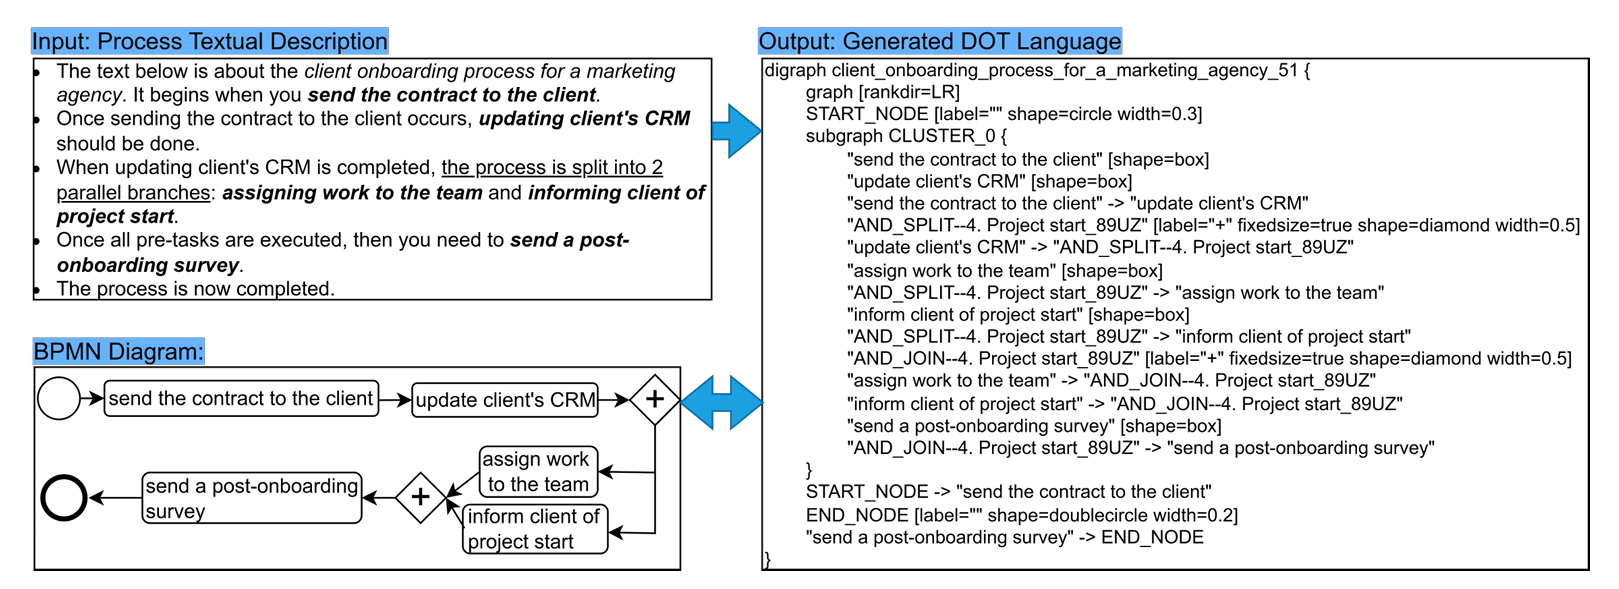
\includegraphics[width=\linewidth]{figures/li2025_text2bpmn_dot.png}
\caption{Text-to-DOT-to-BPMN pipeline example (reproduced from Li et al.\ \cite{li-etal-2025-llm-based-business}).}
\label{fig:li2025-pipeline}
\end{figure}

\paragraph{Task formalization (core equations).}
For a textual business process description $T=\{t_1,\dots,t_n\}$, the model $L$ generates a DOT graph
$D=\{N,E\}$ with node set $N=\{n_1,\dots,n_k\}$ (events, activities, gateways) and edges
$E=\{e_{i,j}\mid n_i,n_j\in N\}$ (sequence flows). Li et al.\ formalize: \cite{li-etal-2025-llm-based-business}
\begin{equation}
L(T;P)=D
\end{equation}
where $P$ denotes the prompting/fine-tuning strategy set. The DOT output is then executed/rendered via a local executor:
\begin{equation}
G=\mathrm{LocalExecution}(D,E)
\end{equation}

\paragraph{Dataset (MaD) and categories.}
They evaluate on the publicly available MaD dataset introduced by Li et al.\ (2023)
and released online as a text--BPMN benchmark \cite{li-etal-2023-mad,li-etal-2023-mad-data},
with text--BPMN pairs across 15 business categories (Table~\ref{tab:li2025-mad-categories}). \cite{li-etal-2025-llm-based-business}


\begin{table}[t]
\centering
\small
\setlength{\tabcolsep}{5pt}
\renewcommand{\arraystretch}{1.12}
\begin{tabular}{@{}ll@{}}
\toprule
\textbf{Abbrev.} & \textbf{Full name} \\
\midrule
APP   & Accounts Payable Process \\
ARP   & Accounts Receivable Process \\
BPP   & Budget Preparation Process \\
CRPP  & Churn Rate Prevention Process \\
COPMA & Client Onboarding Process for Marketing Agency \\
CPP   & Content Promotion Process \\
CSPTM & Customer Support Process for the Ticket Management \\
EOP   & Employee Onboarding Process \\
FGSP  & Final Grades Submission Process \\
LAP   & Loan Application Process \\
OFP   & Order Fulfillment Process \\
POP   & Process for Optimizing a Process \\
PMP   & Project Management Process \\
POW   & Purchase Order Workflow \\
SDDVC & Startup Due Diligence for Venture Capitalist \\
\bottomrule
\end{tabular}
\caption{Business process categories in the MaD dataset (Li et al.).}
\label{tab:li2025-mad-categories}
\end{table}

\paragraph{Hard syntax checking (compilation validity).}
A central automatic gate in their evaluation is \textbf{syntactic validity} of DOT (compile/render success).
They report DOT compilation error rates in Table~\ref{tab:li2025-syntax}. \cite{li-etal-2025-llm-based-business}

\begin{table}[t]
\centering
\small
\setlength{\tabcolsep}{6pt}
\renewcommand{\arraystretch}{1.15}
\begin{tabular}{@{}lccccc@{}}
\toprule
\textbf{Method} & Zero-shot & Zero-shot CoT & Few-shot & Few-shot CoT & Fine-tuned \\
\midrule
Syntax error rate & 6.1\% & 3.7\% & 1.7\% & 0.43\% & 0\% \\
\bottomrule
\end{tabular}
\caption{DOT syntax error rates reported by Li et al.}
\label{tab:li2025-syntax}
\end{table}

\paragraph{Structural and semantic similarity (automatic metrics).}
Beyond syntax, they evaluate (i) \emph{node/label semantics} via sentence embeddings and cosine similarity,
and (ii) \emph{graph structure} via graph embeddings (node2vec) to compare generated graphs against references. \cite{li-etal-2025-llm-based-business}
A common cosine similarity definition is:
\begin{equation}
\mathrm{cos}(u,v)=\frac{u^\top v}{\left\|u\right\|\,\left\|v\right\|}
\end{equation}

\paragraph{Relevance for validity gates.}
Li et al.\ already implement a \emph{syntax gate} (DOT compile success) and \emph{quality checks} (semantic/structural similarity),
but these are not guarantees of BPMN correctness, compliance, or global invariants. This gap motivates deterministic
validity gates (grammar/schema constraints, rule engines, SMT constraints, privacy/PII filters).

% ============================================================
\subsection{A Static Compliance-Checking Framework for Business Process Models (Liu et al., 2007)}
\label{subsec:lmx07-static-compliance}

Liu et al.\ \cite{LMX07} address the enterprise need to automatically verify whether business process models
comply with regulatory constraints before deployment.
The core idea is to keep \emph{process models} and \emph{compliance concerns} separately modeled, then transform both
into formal representations that enable \emph{static verification} via model checking.

\paragraph{High-level pipeline (six steps).}
The method consists of six steps (Figure~\ref{fig:lmx07-method}): (1) model the process in BPEL,
(2) model compliance rules in a visual notation (BPSL), (3.1) transform BPEL into $\pi$-calculus, (3.2) transform
$\pi$-calculus into a finite-state machine (FSM), (4) translate BPSL rules into linear temporal logic (LTL),
(5) perform model checking, and (6) feed counterexamples back to the process layer \cite{LMX07}.

\begin{figure}[t]
\centering
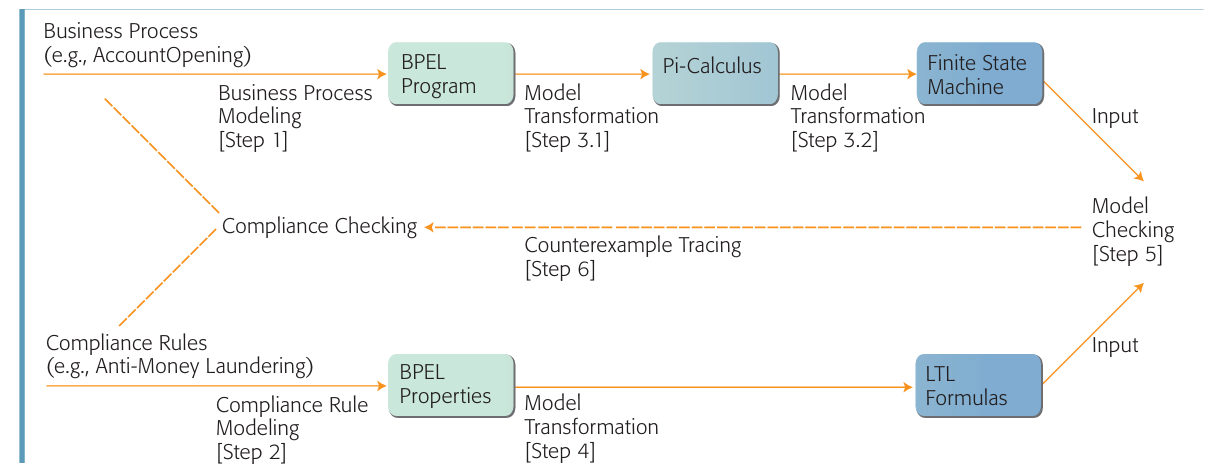
\includegraphics[width=\linewidth]{figures/lmx07_method_overview.png}
\caption{Overview of the static compliance-checking method: BPEL $\rightarrow$ $\pi$-calculus $\rightarrow$ FSM and BPSL $\rightarrow$ LTL, followed by model checking and counterexample tracing \cite{LMX07}.}
\label{fig:lmx07-method}
\end{figure}

\paragraph{Formalization as transformations + model checking.}
The approach can be summarized as a pair of transformations and a verification query:
\begin{align}
\textbf{Process:}\quad & \mathrm{BPEL} \;\xrightarrow{\;\tau_{1}\;}\; \pi\text{-calculus} \;\xrightarrow{\;\tau_{2}\;}\; \mathrm{FSM} \label{eq:lmx07-proc-transform}\\
\textbf{Rules:}\quad & \mathrm{BPSL} \;\xrightarrow{\;\rho\;}\; \mathrm{LTL} \label{eq:lmx07-rule-transform}\\
\textbf{Check:}\quad & \mathrm{FSM} \models \varphi \quad\text{or}\quad \mathrm{FSM} \not\models \varphi \Rightarrow \sigma \label{eq:lmx07-model-check}
\end{align}
where $\varphi$ is the LTL formula derived from the compliance rule model and $\sigma$ is a counterexample trace
(an execution order that violates the rule) \cite{LMX07}.

\paragraph{Why $\pi$-calculus is used (intuitively).}
$\pi$-calculus is a formal model for \emph{concurrent, communicating processes}.
BPEL workflows contain parallelism and message-based interactions; using $\pi$-calculus as an intermediate representation
makes such behaviors explicit and amenable to formal transformation into a finite-state model for verification \cite{LMX07}.
In short: \emph{BPEL is an executable workflow language; $\pi$-calculus provides a mathematically precise semantics for its concurrency and communication constructs.}

\paragraph{$\pi$-calculus syntax (Milner’s polyadic $\pi$-calculus).}
Liu et al.\ adopt Milner’s polyadic $\pi$-calculus as the intermediate formalism and summarize its syntax \cite{LMX07}.
The process grammar is:

\begin{align}
P \;::=&\;\sum_{i=1}^{n} \pi_i . P_i 
\;\mid\; \mathrm{new}\;x\;P 
\;\mid\; P \mid Q 
\;\mid\; !P 
\;\mid\; P / Q
\;\mid\; A(y_1,\dots,y_n) 
\;\mid\; 0 \label{eq:lmx07-pi-proc}\\
\pi \;::=&\;\overline{x}\langle y\rangle \;\mid\; x(y) \;\mid\; \tau \label{eq:lmx07-pi-prefix}\\
\phi \;::=&\;[x = y] \;\mid\; \phi \wedge \phi \;\mid\; \neg \phi \label{eq:lmx07-pi-phi}
\end{align}

\noindent The notation can be interpreted as follows:
(i) $\overline{x}\langle y\rangle$ sends a value $y$ over channel $x$ and $x(y)$ receives a value into variable $y$,
capturing message exchange.
(ii) $P \mid Q$ denotes parallel composition; $!P$ denotes replication (unbounded spawning); and $0$ is the inactive process.
(iii) $\mathrm{new}\;x\;P$ restricts a fresh channel $x$ to process $P$, modeling private communication.
(iv) $\sum_i \pi_i.P_i$ is a guarded choice between possible actions (a form of nondeterministic branching).
This expressiveness is what enables a faithful representation of BPEL control-flow and interaction patterns \cite{LMX07}.

\paragraph{Relevance for validity gates (your thesis angle).}
For LLM-generated automation artifacts, this paper is a blueprint for \emph{deterministic validity gates}:
translate a generated workflow into a formal state-space model (FSM) and translate compliance constraints into a property language (LTL),
then decide acceptance via model checking and return counterexamples as actionable feedback \cite{LMX07}.

% ============================================================
% ============================================================
\subsection{Business Process Compliance Checking: Current State and Future Challenges (El Kharbili et al., 2008)}
\label{subsec:bpcc-kharbili2008}

El Kharbili et al.\ \cite{elkharbili2008bpcc} provide a position paper that surveys business process (BP)
compliance checking in BPM systems and proposes a research agenda motivated by increasing regulatory
and governance demands (e.g., ISO-style quality standards and legislation-driven internal controls).
A central contribution is a structured classification of techniques and a set of open challenges that—while
originating in BPM—translate naturally into \emph{deterministic validity gates} for generated automation artifacts.

\paragraph{Forward vs.\ backward compliance checking.}
The paper distinguishes \emph{backward} compliance checking (post-execution detection using execution histories)
from \emph{forward} compliance checking (design-time or run-time prevention/early detection) \cite{elkharbili2008bpcc}.
Backward techniques can flag non-compliant behavior after the fact but cannot prevent violations; forward techniques
aim to enforce compliance constraints before or during execution.

\begin{figure}[t]
\centering
\begin{tikzpicture}[
  font=\small,
  node distance=6mm and 10mm,
  box/.style={draw, rounded corners=2pt, align=center, inner sep=3.5pt},
  arrow/.style={-Latex, line width=0.9pt},
  dashedarrow/.style={-Latex, dashed, line width=0.9pt}
]
\node (d) [box] {Design-time\\(model)};
\node (dep) [box, right=of d] {Deployment};
\node (rt) [box, right=of dep] {Run-time\\(instances)};
\node (log) [box, right=of rt] {History\\/ Logs};

\draw[arrow] (d) -- node[above]{process lifecycle} (dep);
\draw[arrow] (dep) -- (rt);
\draw[arrow] (rt) -- (log);

\draw[arrow] (d.north) .. controls +(0,10mm) and +(0,10mm) .. node[above]{\textbf{forward compliance} (prevent / enforce)} (rt.north);
\draw[dashedarrow] (log.south) .. controls +(0,-10mm) and +(0,-10mm) .. node[below]{\textbf{backward compliance} (detect)} (rt.south);
\end{tikzpicture}
\caption{Compliance checking taxonomy in \cite{elkharbili2008bpcc}: forward (design-/run-time) vs.\ backward (post-execution log-based).}
\label{fig:bpcc-forward-backward}
\end{figure}

\paragraph{Representative technique families.}
In the surveyed landscape, multiple formalizations are used to encode compliance constraints:
(i) \emph{static compliance checking} of process models against compliance rules \cite{LMX07},
(ii) \emph{policy-/deontic-/contract-based} formalisms treating BPs as normative interaction processes
(e.g., deontic assignments and contract logics) \cite{PR,Mil05b,GG06,GZ05,MOS06,SGN07},
(iii) \emph{pattern-based} compliance design and validation using reusable control patterns and semantic layers
\cite{NS07a,NS07b,NS08},
(iv) \emph{run-time compliance checking} requiring execution data, including temporal-logic specifications and
formal execution semantics (e.g., BPEL-to-$\pi$-calculus plus temporal logic) \cite{Mi93,DF06,GH01},
and (v) \emph{conformance checking} that compares observed event logs against the intended control-flow model
\cite{RA08,ABD05}. The paper notes that several approaches remain limited to control-flow aspects and may be
unable to check constraints involving \emph{data fields} or \emph{performer/organizational} information \cite{elkharbili2008bpcc}.

\paragraph{Key challenges and agenda.}
El Kharbili et al.\ argue that progress is constrained by four recurring gaps \cite{elkharbili2008bpcc}:
\begin{itemize}
  \item \textbf{Lifecycle coverage:} no approach covers the full BPM lifecycle end-to-end (design, deployment, execution, monitoring).
  \item \textbf{Beyond control-flow:} compliance checks should incorporate data, resources, duties (e.g., SoD), and domain-specific standards.
  \item \textbf{Usability:} business analysts are the primary target users, yet many formalisms remain too technical; intuitive graphical notations are needed.
  \item \textbf{Semantics:} semantic technologies (e.g., compliance ontologies) are needed to reduce ambiguity in natural-language regulations and to
  support declarative, policy-based compliance checking \cite{SBO07,LGRMD08,FY07}.
\end{itemize}

\paragraph{Relevance for validity gates in LLM-generated automation.}
From a validity-gate perspective, the paper provides a mature reference frame:
\emph{hard acceptance criteria} arise from formal constraint languages (temporal logic, deontic/policy rules, patterns, ontologies),
while execution-time evidence comes from logs and monitoring. This directly supports a gate architecture in which an LLM proposes
automation artifacts, but compliance is \emph{deterministically decided} by external checkers across phases (design-time validation,
run-time enforcement, and backward conformance analysis) \cite{elkharbili2008bpcc,ABD05,RA08,SGN07}.

% ============================================================
\subsection{De-Identifying Student Personally Identifying Information with GPT-4 (Singhal et al., EDM 2024)}
\label{subsec:deid-gpt4-edm2024}

Singhal et al.\ \cite{singhal2024deid_gpt4} evaluate whether GPT-4 can be used as a practical tool
to de-identify student-generated text by redacting personally identifying information (PII) in discussion
forum posts from nine Massive Open Online Courses (MOOCs).
The motivation is compliance with privacy regulations (e.g., GDPR) and the need to safely release datasets
for open science while preserving participant confidentiality \cite{singhal2024deid_gpt4}.

\paragraph{Setting and process.}
The authors apply GPT-4 to redact PII in forum posts and treat \emph{human redaction} as ground truth for evaluation.
They report that the system can also identify PII cases missed by human coders, but exhibits substantial
\emph{over-redaction} (false positives), especially for names and locations that do not constitute PII in context
\cite{singhal2024deid_gpt4}.
The paper states that forum posts were sent individually to the OpenAI \texttt{gpt-4-0613} API with
\texttt{max\_tokens}=1000 and otherwise default parameters, and discusses data handling under the provider’s
policy at the time of the study \cite{singhal2024deid_gpt4}.

\paragraph{Dataset distribution (nine courses).}
Table~\ref{tab:deid-gpt4-dist} summarizes the distribution of posts and redactions across courses
after corrections, including the fraction of posts containing at least one redacted element and how often
PII was initially missed by humans \cite{singhal2024deid_gpt4}.

\begin{table}[t]
\centering
\small
\setlength{\tabcolsep}{5pt}
\renewcommand{\arraystretch}{1.08}
\begin{tabular}{@{}l l r r r r r@{}}
\toprule
\textbf{Course} & \textbf{Topic} & \textbf{Total} & \textbf{Posts w/} & \textbf{Words/} & \textbf{Redacted} & \textbf{PII missed} \\
 &  & \textbf{Posts} & \textbf{Redactions} & \textbf{Post} & \textbf{Words} & \textbf{by humans} \\
\midrule
Accounting &  & 387 & 165 (42.6\%) & 47.0  & 251 (1.4\%) & 6 (3.6\%) \\
Calculus  &  & 396 & 114 (28.8\%) & 40.0  & 162 (1.0\%) & 3 (2.6\%) \\
Design    &  & 380 & 194 (51.1\%) & 44.4  & 283 (1.7\%) & 8 (4.1\%) \\
Gamification &  & 379 & 124 (32.7\%) & 63.5 & 237 (1.0\%) & 7 (5.6\%) \\
Business trends &  & 387 & 143 (37.0\%) & 81.1 & 291 (0.9\%) & 15 (10.5\%) \\
Poetry    &  & 399 & 85 (21.3\%)  & 241.0 & 124 (0.1\%) & 2 (2.4\%) \\
Mythology &  & 390 & 138 (35.4\%) & 67.9 & 196 (0.7\%) & 1 (0.7\%) \\
Probability &  & 396 & 117 (29.5\%) & 56.9 & 177 (0.8\%) & 0 (0\%) \\
Vaccines  &  & 391 & 159 (40.7\%) & 71.2 & 287 (1.0\%) & 3 (1.9\%) \\
\bottomrule
\end{tabular}
\caption{Distribution of posts and redacted elements across the nine MOOCs (reported in \cite{singhal2024deid_gpt4}).}
\label{tab:deid-gpt4-dist}
\end{table}

\paragraph{Performance (precision--recall trade-off).}
Table~\ref{tab:deid-gpt4-metrics} reports precision, recall, and inter-rater agreement (Cohen’s $\kappa$)
for each course when using human redaction as ground truth \cite{singhal2024deid_gpt4}.
The key result is a high average recall of 0.958, indicating that GPT-4 identifies most PII instances that should
be redacted, but substantially lower average precision of 0.526, indicating frequent over-redaction.

\begin{table}[t]
\centering
\small
\setlength{\tabcolsep}{6pt}
\renewcommand{\arraystretch}{1.08}
\begin{tabular}{@{}l c c c@{}}
\toprule
\textbf{Course} & \textbf{Precision} & \textbf{Recall} & \textbf{$\kappa$} \\
\midrule
Accounting      & 0.716 & 0.975 & 0.823 \\
Calculus        & 0.666 & 0.922 & 0.771 \\
Design          & 0.742 & 0.984 & 0.843 \\
Gamification    & 0.658 & 0.967 & 0.780 \\
Business trends & 0.366 & 0.983 & 0.527 \\
Poetry          & 0.158 & 0.895 & 0.267 \\
Mythology       & 0.374 & 0.937 & 0.530 \\
Probability     & 0.602 & 0.988 & 0.763 \\
Vaccines        & 0.454 & 0.966 & 0.612 \\
\midrule
\textbf{Average} & \textbf{0.526} & \textbf{0.958} & \textbf{0.657} \\
\bottomrule
\end{tabular}
\caption{Performance metrics of GPT-4 de-identification using human redaction as ground truth (reported in \cite{singhal2024deid_gpt4}).}
\label{tab:deid-gpt4-metrics}
\end{table}

\paragraph{Comparison to prior de-identification approaches.}
Table~\ref{tab:deid-gpt4-compare} compares GPT-4 to representative de-identification methods from prior work as summarized
by the authors \cite{singhal2024deid_gpt4}. While some supervised approaches outperform GPT-4, the paper notes that direct
comparisons are complicated by differences in targeted PII types and task scope (e.g., focusing exclusively on names).

\begin{table}[t]
\centering
\small
\setlength{\tabcolsep}{6pt}
\renewcommand{\arraystretch}{1.10}
\begin{tabular}{@{}l l l c c@{}}
\toprule
\textbf{Work} & \textbf{PII} & \textbf{Method} & \textbf{Precision} & \textbf{Recall} \\
\midrule
Bosch et al.  & Names & ExtraTrees + Deep Neural Nets & 0.827 & 0.970 \\
Farrow et al. & Names & RegEx & 0.550 & 0.905 \\
Holmes et al. & Names & Fine-tuned RoBERTa & 0.680 & 0.840 \\
\textbf{This paper} & Names, Locations, Links & GPT-4 & 0.526 & 0.958 \\
\bottomrule
\end{tabular}
\caption{Comparison to selected de-identification methods (as reported in \cite{singhal2024deid_gpt4}).}
\label{tab:deid-gpt4-compare}
\end{table}

\paragraph{Implications for validity gates.}
From a validity-gate perspective, the main lesson is the \emph{precision--recall trade-off}:
high recall is attractive for compliance-critical pipelines (minimizing leakage), but low precision can reduce utility
by over-redacting benign entities \cite{singhal2024deid_gpt4}. This supports gate designs that combine deterministic pattern-based
filters (for well-defined PII types) with LLM-based redaction as an additional, probabilistic layer and explicit escalation policies
for ambiguous cases.

% ============================================================
\subsection{JSONSchemaBench: Benchmarking Constrained Decoding for Structured Outputs}
\label{subsec:jsonschemabench}

Constrained decoding has emerged as a dominant mechanism for enforcing \emph{structured outputs} during LLM generation by masking invalid tokens with respect to a target constraint language (e.g., JSON Schema). JSONSchemaBench \cite{geng2025jsonschemabench} contributes a rigorous benchmark and evaluation framework for comparing constrained-decoding systems along three dimensions:
\textbf{(Q1) efficiency} (runtime overhead or speedup), \textbf{(Q2) coverage} (support for real-world schema features), and \textbf{(Q3) quality} (impact on downstream task performance).

\paragraph{Benchmark and evaluated frameworks.}
JSONSchemaBench \cite{geng2025jsonschemabench} comprises \textbf{10K real-world JSON Schemas} spanning a wide variety of constraint types and complexities. The benchmark is paired with the \emph{official JSON Schema Test Suite}. The authors evaluate multiple state-of-the-art constrained-decoding frameworks (including Guidance, Outlines, llama.cpp grammar module, XGrammar, and hosted model interfaces) to uncover practical trade-offs between speed, feature support, and output quality.

\paragraph{Key findings (high-level).}
Across extensive experiments, the authors report three central results (illustrated in Figure~\ref{fig:jsonschemabench-fig1}):
(1) constrained decoding can \emph{speed up} generation by up to \textbf{50\%} compared to LM-only decoding,
(2) practical support for real-world schemas varies strongly across frameworks (best supports about \textbf{2$\times$} as many schemas as worst),
and (3) constrained decoding can \emph{improve} downstream performance by up to \textbf{4\%}, even on tasks with minimal structure (e.g., GSM8k), indicating that constraints can act as a beneficial inductive bias rather than merely an overhead \cite{geng2025jsonschemabench}.

\begin{figure}[t]
\centering
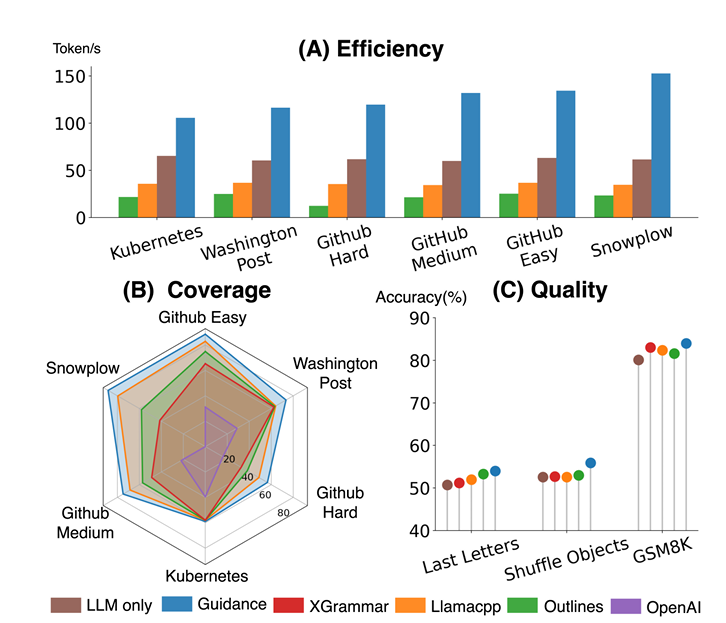
\includegraphics[width=0.92\linewidth]{figures/jsonschemabench_fig1.png}
\caption{Efficiency--coverage--quality comparison across constrained-decoding frameworks (adapted from \cite{geng2025jsonschemabench}).}
\label{fig:jsonschemabench-fig1}
\end{figure}

\paragraph{Efficiency metrics.}
The evaluation decomposes efficiency into:
\textbf{Grammar Compilation Time (GCT)}, \textbf{Time to First Token (TTFT)}, and \textbf{Time per Output Token (TPOT)} \cite{geng2025jsonschemabench}.
Table~\ref{tab:jsonschemabench-eff-llamacpp} shows representative median efficiency measurements with llama.cpp as inference engine.
A notable qualitative takeaway is that Guidance and llama.cpp compute constraints dynamically with negligible compilation overhead, whereas Outlines exhibits substantial compilation costs due to schema-to-regex-style conversions \cite{geng2025jsonschemabench}.

\begin{table}[t]
\centering
\small
\setlength{\tabcolsep}{6pt}
\renewcommand{\arraystretch}{1.12}
\begin{tabular}{@{}l l c c c@{}}
\toprule
\textbf{Dataset} & \textbf{Framework} & \textbf{GCT (s)} & \textbf{TTFT (s)} & \textbf{TPOT (ms)} \\
\midrule
GlaiveAI      & LM-only   & --   & 0.10 & 15.40 \\
              & Guidance  & 0.00 & 0.24 & 6.37  \\
              & Llamacpp  & 0.05 & 0.20 & 29.98 \\
              & Outlines  & 3.48 & 3.65 & 30.33 \\
\midrule
GitHub Easy   & LM-only   & --   & 0.10 & 15.83 \\
              & Guidance  & 0.00 & 0.34 & 7.44  \\
              & Llamacpp  & 0.05 & 0.18 & 27.22 \\
              & Outlines  & 3.71 & 3.97 & 39.78 \\
\midrule
Snowplow      & LM-only   & --   & 0.11 & 16.23 \\
              & Guidance  & 0.00 & 0.28 & 6.55  \\
              & Llamacpp  & 0.05 & 0.20 & 28.90 \\
              & Outlines  & 3.91 & 4.14 & 42.66 \\
\midrule
GitHub Medium & LM-only   & --   & 0.20 & 16.68 \\
              & Guidance  & 0.01 & 0.54 & 7.57  \\
              & Llamacpp  & 0.06 & 0.30 & 29.08 \\
              & Outlines  & 8.05 & 8.38 & 46.57 \\
\midrule
Kubernetes    & LM-only   & --   & 0.16 & 15.32 \\
              & Guidance  & 0.01 & 0.45 & 9.47  \\
              & Llamacpp  & 0.05 & 0.28 & 28.04 \\
              & Outlines  & 5.29 & 5.55 & 46.10 \\
\bottomrule
\end{tabular}
\caption{Efficiency metrics reported in JSONSchemaBench with llama.cpp as inference engine (median values). GCT: grammar compilation time, TTFT: time to first token, TPOT: time per output token \cite{geng2025jsonschemabench}.}
\label{tab:jsonschemabench-eff-llamacpp}
\end{table}

Because XGrammar does not support llama.cpp, the authors additionally compare XGrammar vs.\ Guidance under a Hugging Face Transformers backend (Table~\ref{tab:jsonschemabench-eff-hf}) \cite{geng2025jsonschemabench}.

\begin{table}[t]
\centering
\small
\setlength{\tabcolsep}{6pt}
\renewcommand{\arraystretch}{1.12}
\begin{tabular}{@{}l l c c c@{}}
\toprule
\textbf{Dataset} & \textbf{Framework} & \textbf{GCT (s)} & \textbf{TTFT (s)} & \textbf{TPOT (ms)} \\
\midrule
GlaiveAI      & Guidance & 0.01 & 0.36 & 36.92 \\
              & XGrammar & 0.12 & 0.30 & 66.78 \\
\midrule
GitHub Easy   & Guidance & 0.01 & 0.37 & 42.03 \\
              & XGrammar & 0.11 & 0.33 & 65.57 \\
\midrule
GitHub Medium & Guidance & 0.01 & 0.55 & 44.21 \\
              & XGrammar & 0.20 & 0.48 & 65.51 \\
\midrule
GitHub Hard   & Guidance & 0.01 & 0.73 & 35.88 \\
              & XGrammar & 0.30 & 0.65 & 65.20 \\
\bottomrule
\end{tabular}
\caption{Additional efficiency experiment with Hugging Face Transformers backend for Guidance vs.\ XGrammar (median values) \cite{geng2025jsonschemabench}.}
\label{tab:jsonschemabench-eff-hf}
\end{table}

\paragraph{Coverage: declared, empirical, and true.}
A distinctive contribution of JSONSchemaBench is a fine-grained coverage taxonomy \cite{geng2025jsonschemabench}:
\begin{itemize}
  \item \textbf{Declared coverage:} the framework processes a schema without explicit rejection or runtime errors.
  \item \textbf{Empirical coverage:} generated constraints yield outputs that are schema-compliant in experiments.
  \item \textbf{True coverage:} generated constraints are precisely equivalent to the original schema (accept all compliant outputs and reject all noncompliant ones).
\end{itemize}
This separation is crucial for validity gates: a system may accept a schema (declared) yet still under-constrain or over-constrain it in practice.

Table~\ref{tab:jsonschemabench-coverage} summarizes coverage across schema categories at increasing thresholds. A key outcome is that Guidance achieves substantially higher coverage across thresholds than other evaluated engines \cite{geng2025jsonschemabench}.

\begin{table}[t]
\centering
\small
\setlength{\tabcolsep}{6pt}
\renewcommand{\arraystretch}{1.12}
\begin{tabular}{@{}l c c c c@{}}
\toprule
\textbf{Coverage threshold (categories)} & \textbf{Outlines} & \textbf{Llamacpp} & \textbf{XGrammar} & \textbf{Guidance} \\
\midrule
Minimal coverage ($>0\%$)   & 20 & 21 & 28 & \textbf{30} \\
Partial coverage ($>25\%$)  & 11 & 11 & 16 & \textbf{25} \\
Moderate coverage ($>50\%$) &  2 &  5 &  3 & \textbf{21} \\
High coverage ($>75\%$)     &  0 &  2 &  1 & \textbf{17} \\
Full coverage ($100\%$)     &  0 &  1 &  1 & \textbf{13} \\
Tied for highest ($>0\%$)   &  4 &  6 & 14 & \textbf{25} \\
Single highest              &  1 &  0 & 10 & \textbf{19} \\
\bottomrule
\end{tabular}
\caption{Coverage by schema categories at increasing thresholds (reported in \cite{geng2025jsonschemabench}).}
\label{tab:jsonschemabench-coverage}
\end{table}

\paragraph{Failure modes: compile errors vs.\ over-/under-constraining.}
Beyond aggregate coverage, the benchmark identifies recurring failure types, which are directly relevant for enterprise-grade gates: compile-time errors, \emph{over-constrained} constraints (reject valid outputs), and \emph{under-constrained} constraints (accept invalid outputs). Table~\ref{tab:jsonschemabench-failures} reports how many categories exhibited each failure at least once. Under-constraining is particularly critical for compliance, since it may create a false sense of safety \cite{geng2025jsonschemabench}.

\begin{table}[t]
\centering
\small
\setlength{\tabcolsep}{6pt}
\renewcommand{\arraystretch}{1.12}
\begin{tabular}{@{}l c c c c@{}}
\toprule
\textbf{Failure type} & \textbf{Outlines} & \textbf{Llamacpp} & \textbf{XGrammar} & \textbf{Guidance} \\
\midrule
CompileError     & 42 & 37 & \textbf{3}  & 25 \\
Over-constrained & 16 & 18 & 5  & \textbf{7} \\
Under-constrained&  8 &  7 & 38 & \textbf{1} \\
\bottomrule
\end{tabular}
\caption{Number of categories with at least one occurrence of each failure type (reported in \cite{geng2025jsonschemabench}).}
\label{tab:jsonschemabench-failures}
\end{table}

\paragraph{Implication for validity-gate design.}
JSONSchemaBench \cite{geng2025jsonschemabench} provides a concrete blueprint for evaluating validity gates beyond mere ``schema pass rate'':
a gate must be assessed for \emph{efficiency} (deployability), \emph{coverage} (real-world constraint support), and \emph{quality impact}.
Moreover, the declared/empirical/true coverage distinction and over-/under-constraining failure modes directly inform how a gate should be logged and audited in enterprise pipelines.

% ============================================================
\subsection{JSONSchemaBench: Benchmarking Constrained Decoding for Structured Outputs}
\label{subsec:jsonschemabench}

Constrained decoding has emerged as a dominant mechanism for enforcing \emph{structured outputs} during LLM generation by masking invalid tokens with respect to a target constraint language (e.g., JSON Schema). JSONSchemaBench \cite{geng2025jsonschemabench} contributes a rigorous benchmark and evaluation framework for comparing constrained-decoding systems along three dimensions:
\textbf{(Q1) efficiency} (runtime overhead or speedup), \textbf{(Q2) coverage} (support for real-world schema features), and \textbf{(Q3) quality} (impact on downstream task performance).

\paragraph{Benchmark and evaluated frameworks.}
JSONSchemaBench \cite{geng2025jsonschemabench} comprises \textbf{10K real-world JSON Schemas} spanning a wide variety of constraint types and complexities. The benchmark is paired with the \emph{official JSON Schema Test Suite}. The authors evaluate multiple state-of-the-art constrained-decoding frameworks (including Guidance, Outlines, llama.cpp grammar module, XGrammar, and hosted model interfaces) to uncover practical trade-offs between speed, feature support, and output quality.

\paragraph{Key findings (high-level).}
Across extensive experiments, the authors report three central results (illustrated in Figure~\ref{fig:jsonschemabench-fig1}):
(1) constrained decoding can \emph{speed up} generation by up to \textbf{50\%} compared to LM-only decoding,
(2) practical support for real-world schemas varies strongly across frameworks (best supports about \textbf{2$\times$} as many schemas as worst),
and (3) constrained decoding can \emph{improve} downstream performance by up to \textbf{4\%}, even on tasks with minimal structure (e.g., GSM8k), indicating that constraints can act as a beneficial inductive bias rather than merely an overhead \cite{geng2025jsonschemabench}.

\begin{figure}[t]
\centering
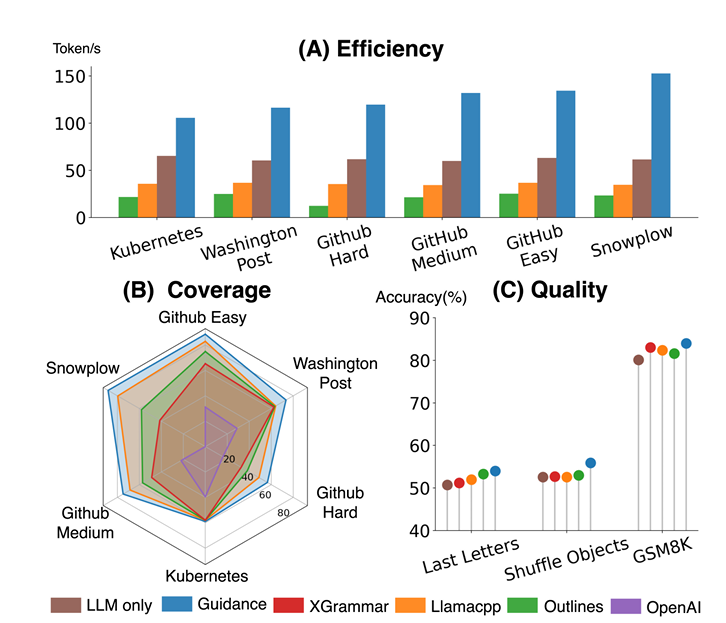
\includegraphics[width=0.92\linewidth]{figures/jsonschemabench_fig1.png}
\caption{Efficiency--coverage--quality comparison across constrained-decoding frameworks (adapted from \cite{geng2025jsonschemabench}).}
\label{fig:jsonschemabench-fig1}
\end{figure}

\paragraph{Efficiency metrics.}
The evaluation decomposes efficiency into:
\textbf{Grammar Compilation Time (GCT)}, \textbf{Time to First Token (TTFT)}, and \textbf{Time per Output Token (TPOT)} \cite{geng2025jsonschemabench}.
Table~\ref{tab:jsonschemabench-eff-llamacpp} shows representative median efficiency measurements with llama.cpp as inference engine.
A notable qualitative takeaway is that Guidance and llama.cpp compute constraints dynamically with negligible compilation overhead, whereas Outlines exhibits substantial compilation costs due to schema-to-regex-style conversions \cite{geng2025jsonschemabench}.

\begin{table}[t]
\centering
\small
\setlength{\tabcolsep}{6pt}
\renewcommand{\arraystretch}{1.12}
\begin{tabular}{@{}l l c c c@{}}
\toprule
\textbf{Dataset} & \textbf{Framework} & \textbf{GCT (s)} & \textbf{TTFT (s)} & \textbf{TPOT (ms)} \\
\midrule
GlaiveAI      & LM-only   & --   & 0.10 & 15.40 \\
              & Guidance  & 0.00 & 0.24 & 6.37  \\
              & Llamacpp  & 0.05 & 0.20 & 29.98 \\
              & Outlines  & 3.48 & 3.65 & 30.33 \\
\midrule
GitHub Easy   & LM-only   & --   & 0.10 & 15.83 \\
              & Guidance  & 0.00 & 0.34 & 7.44  \\
              & Llamacpp  & 0.05 & 0.18 & 27.22 \\
              & Outlines  & 3.71 & 3.97 & 39.78 \\
\midrule
Snowplow      & LM-only   & --   & 0.11 & 16.23 \\
              & Guidance  & 0.00 & 0.28 & 6.55  \\
              & Llamacpp  & 0.05 & 0.20 & 28.90 \\
              & Outlines  & 3.91 & 4.14 & 42.66 \\
\midrule
GitHub Medium & LM-only   & --   & 0.20 & 16.68 \\
              & Guidance  & 0.01 & 0.54 & 7.57  \\
              & Llamacpp  & 0.06 & 0.30 & 29.08 \\
              & Outlines  & 8.05 & 8.38 & 46.57 \\
\midrule
Kubernetes    & LM-only   & --   & 0.16 & 15.32 \\
              & Guidance  & 0.01 & 0.45 & 9.47  \\
              & Llamacpp  & 0.05 & 0.28 & 28.04 \\
              & Outlines  & 5.29 & 5.55 & 46.10 \\
\bottomrule
\end{tabular}
\caption{Efficiency metrics reported in JSONSchemaBench with llama.cpp as inference engine (median values). GCT: grammar compilation time, TTFT: time to first token, TPOT: time per output token \cite{geng2025jsonschemabench}.}
\label{tab:jsonschemabench-eff-llamacpp}
\end{table}

Because XGrammar does not support llama.cpp, the authors additionally compare XGrammar vs.\ Guidance under a Hugging Face Transformers backend (Table~\ref{tab:jsonschemabench-eff-hf}) \cite{geng2025jsonschemabench}.

\begin{table}[t]
\centering
\small
\setlength{\tabcolsep}{6pt}
\renewcommand{\arraystretch}{1.12}
\begin{tabular}{@{}l l c c c@{}}
\toprule
\textbf{Dataset} & \textbf{Framework} & \textbf{GCT (s)} & \textbf{TTFT (s)} & \textbf{TPOT (ms)} \\
\midrule
GlaiveAI      & Guidance & 0.01 & 0.36 & 36.92 \\
              & XGrammar & 0.12 & 0.30 & 66.78 \\
\midrule
GitHub Easy   & Guidance & 0.01 & 0.37 & 42.03 \\
              & XGrammar & 0.11 & 0.33 & 65.57 \\
\midrule
GitHub Medium & Guidance & 0.01 & 0.55 & 44.21 \\
              & XGrammar & 0.20 & 0.48 & 65.51 \\
\midrule
GitHub Hard   & Guidance & 0.01 & 0.73 & 35.88 \\
              & XGrammar & 0.30 & 0.65 & 65.20 \\
\bottomrule
\end{tabular}
\caption{Additional efficiency experiment with Hugging Face Transformers backend for Guidance vs.\ XGrammar (median values) \cite{geng2025jsonschemabench}.}
\label{tab:jsonschemabench-eff-hf}
\end{table}

\paragraph{Coverage: declared, empirical, and true.}
A distinctive contribution of JSONSchemaBench is a fine-grained coverage taxonomy \cite{geng2025jsonschemabench}:
\begin{itemize}
  \item \textbf{Declared coverage:} the framework processes a schema without explicit rejection or runtime errors.
  \item \textbf{Empirical coverage:} generated constraints yield outputs that are schema-compliant in experiments.
  \item \textbf{True coverage:} generated constraints are precisely equivalent to the original schema (accept all compliant outputs and reject all noncompliant ones).
\end{itemize}
This separation is crucial for validity gates: a system may accept a schema (declared) yet still under-constrain or over-constrain it in practice.

Table~\ref{tab:jsonschemabench-coverage} summarizes coverage across schema categories at increasing thresholds. A key outcome is that Guidance achieves substantially higher coverage across thresholds than other evaluated engines \cite{geng2025jsonschemabench}.

\begin{table}[t]
\centering
\small
\setlength{\tabcolsep}{6pt}
\renewcommand{\arraystretch}{1.12}
\begin{tabular}{@{}l c c c c@{}}
\toprule
\textbf{Coverage threshold (categories)} & \textbf{Outlines} & \textbf{Llamacpp} & \textbf{XGrammar} & \textbf{Guidance} \\
\midrule
Minimal coverage ($>0\%$)   & 20 & 21 & 28 & \textbf{30} \\
Partial coverage ($>25\%$)  & 11 & 11 & 16 & \textbf{25} \\
Moderate coverage ($>50\%$) &  2 &  5 &  3 & \textbf{21} \\
High coverage ($>75\%$)     &  0 &  2 &  1 & \textbf{17} \\
Full coverage ($100\%$)     &  0 &  1 &  1 & \textbf{13} \\
Tied for highest ($>0\%$)   &  4 &  6 & 14 & \textbf{25} \\
Single highest              &  1 &  0 & 10 & \textbf{19} \\
\bottomrule
\end{tabular}
\caption{Coverage by schema categories at increasing thresholds (reported in \cite{geng2025jsonschemabench}).}
\label{tab:jsonschemabench-coverage}
\end{table}

\paragraph{Failure modes: compile errors vs.\ over-/under-constraining.}
Beyond aggregate coverage, the benchmark identifies recurring failure types, which are directly relevant for enterprise-grade gates: compile-time errors, \emph{over-constrained} constraints (reject valid outputs), and \emph{under-constrained} constraints (accept invalid outputs). Table~\ref{tab:jsonschemabench-failures} reports how many categories exhibited each failure at least once. Under-constraining is particularly critical for compliance, since it may create a false sense of safety \cite{geng2025jsonschemabench}.

\begin{table}[t]
\centering
\small
\setlength{\tabcolsep}{6pt}
\renewcommand{\arraystretch}{1.12}
\begin{tabular}{@{}l c c c c@{}}
\toprule
\textbf{Failure type} & \textbf{Outlines} & \textbf{Llamacpp} & \textbf{XGrammar} & \textbf{Guidance} \\
\midrule
CompileError     & 42 & 37 & \textbf{3}  & 25 \\
Over-constrained & 16 & 18 & 5  & \textbf{7} \\
Under-constrained&  8 &  7 & 38 & \textbf{1} \\
\bottomrule
\end{tabular}
\caption{Number of categories with at least one occurrence of each failure type (reported in \cite{geng2025jsonschemabench}).}
\label{tab:jsonschemabench-failures}
\end{table}

\paragraph{Implication for validity-gate design.}
JSONSchemaBench \cite{geng2025jsonschemabench} provides a concrete blueprint for evaluating validity gates beyond mere ``schema pass rate'':
a gate must be assessed for \emph{efficiency} (deployability), \emph{coverage} (real-world constraint support), and \emph{quality impact}.
Moreover, the declared/empirical/true coverage distinction and over-/under-constraining failure modes directly inform how a gate should be logged and audited in enterprise pipelines.

% ============================================================
\subsubsection{Error Checking: Verification Mechanisms During and After Generation}
\label{subsec:error-checking}

\paragraph{Hard syntactic guarantees (constrained decoding and schemas).}
Lexically constrained decoding enforces mandatory phrases or lexical constraints during generation \cite{hokamp2017lexically}.
LLM-focused work extends this to \emph{grammar-constrained decoding}, guaranteeing syntactic validity w.r.t.\ a grammar.
Grammar-aligned decoding aims to preserve model likelihood while maintaining grammatical guarantees \cite{park2024grammaraligned},
and recent work improves efficiency for real grammars \cite{park2025flexible}.
For schema-centric outputs, JSONSchemaBench provides a benchmark methodology to measure schema compliance, efficiency, and quality \cite{geng2025jsonschemabench}.

\paragraph{Probabilistic self-checking and supervision-based verification.}
Chain-of-Verification (CoVe) drafts an answer, creates verification questions, answers them independently, and revises the final output,
reducing hallucinations across benchmarks \cite{dhuliawala2024cove}.
Process supervision improves reasoning reliability by scoring intermediate steps rather than only final answers \cite{lightman2023verify}.
These approaches reduce error rates but do not provide formal per-instance guarantees.

\paragraph{LLM-as-judge as checking baseline.}
G-Eval uses strong models as judges and improves alignment with human judgments \cite{liu2023geval},
while JudgeBench benchmarks judge robustness and highlights failure modes \cite{tan2024judgebench}.

% ============================================================
\subsection{Reasons for Errors: Why ``Deterministic'' LLM Outputs Are Not Reliable}
\label{subsec:reasons}

\subsubsection{Non-Determinism under Deterministic Inference Settings}
\label{subsec:nondeterminism}

A fundamental challenge for deploying LLMs in enterprise and compliance-critical environments is their lack of reproducibility.
Even when inference parameters are configured to be deterministic, repeated executions may yield substantially different outputs.
The work \cite{nondeterminism_llm_settings} systematically studies this phenomenon and reports accuracy variations of up to 15\% across naturally occurring runs.
More strikingly, the gap between the best- and worst-performing runs can reach up to 70\%, highlighting severe instability.

Determinism in LLM inference is commonly associated with the temperature parameter.
Let $y_i$ denote the logit assigned to token $i$ by the model, and let $T$ denote the temperature.
The probability of sampling token $i$ is given by
\begin{equation}
P(i) = \frac{e^{y_i / T}}{\sum_{j=1}^{N} e^{y_j / T}} ,
\label{eq:softmax_temperature}
\end{equation}
where $T=0$ is theoretically expected to yield deterministic behavior.
While increasing $T$ diversifies outputs, \cite{nondeterminism_llm_settings} confirms that other decoding hyperparameters,
such as top-$p$ sampling, have only marginal effects on determinism when temperature is fixed.

To quantify instability, the authors evaluate eight tasks drawn from BIG-Bench Hard (BBH) and MMLU, summarized in Table~\ref{tab:tasks_bbh_mmlu}. \cite{nondeterminism_llm_settings}

\begin{table}[h]
\centering
\small
\begin{tabular}{l l c c}
\hline
\textbf{Benchmark} & \textbf{Task Description} & \textbf{\#Examples} & \textbf{\#Options} \\
\hline
BBH & Navigation (path ends at start) & 250 & 2 \\
BBH & Ruin names (humorous edits) & 250 & 4 \\
BBH & Geometric shapes (SVG) & 250 & 10 \\
BBH & Logical deduction (object ordering) & 250 & 3 \\
MMLU & European history (high school) & 165 & 4 \\
MMLU & College mathematics & 100 & 4 \\
MMLU & Professional accounting & 282 & 4 \\
MMLU & Public relations and media theory & 110 & 4 \\
\hline
\end{tabular}
\caption{Tasks from BBH and MMLU evaluated for non-deterministic behavior \cite{nondeterminism_llm_settings}.}
\label{tab:tasks_bbh_mmlu}
\end{table}

\begin{figure}[h]
\centering
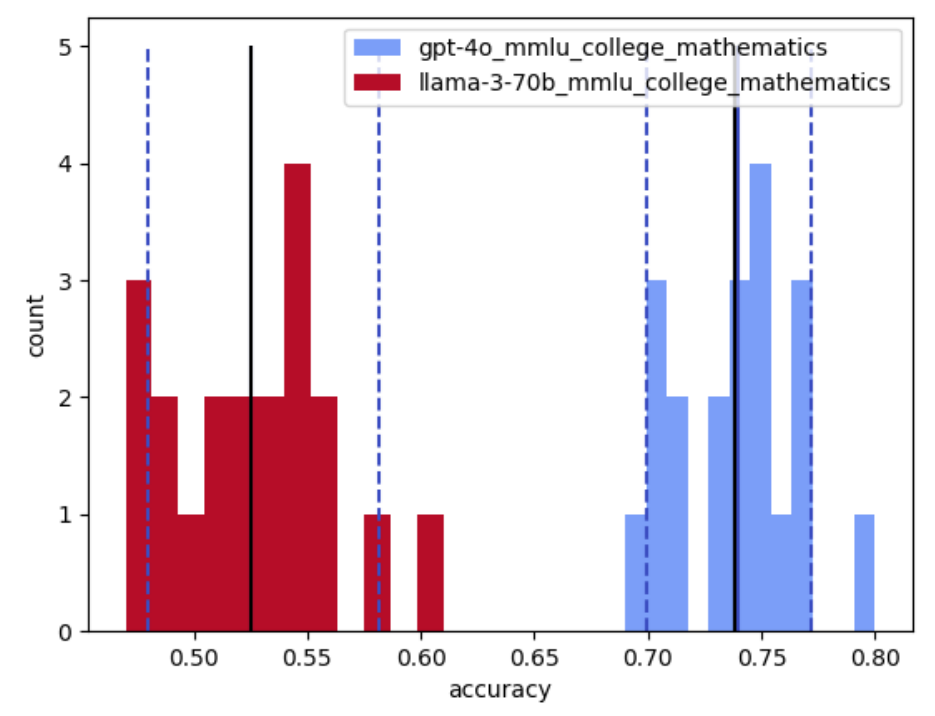
\includegraphics[width=0.7\linewidth]{figures/nondeterminism_accuracy.png}
\caption{Accuracy over 20 identical inference runs on the college mathematics task at $T=0$ \cite{nondeterminism_llm_settings}.}
\label{fig:nondeterminism_accuracy}
\end{figure}

\subsubsection{Memorization and data leakage}
Models can emit memorized training sequences under extraction attacks \cite{carlini2021extracting}, and memorization scales with model and data factors \cite{carlini2022memorization}.
This motivates privacy-oriented output gates (e.g., PII detection/redaction) and stricter data minimization.


% ============================================================
\subsection{Output Validity Gates: Deterministic Acceptance Criteria for Structured and Compliant Artifacts}
\label{subsec:output-validity-gates}

\paragraph{Schema and interface specifications as objective validity criteria.}
JSON Schema specifies machine-checkable constraints for JSON payloads \cite{jsonschema202012}.
OpenAPI defines standardized API contracts aligned with JSON Schema (notably in OpenAPI 3.1+) \cite{openapi31}.
Protocol Buffers and Apache Avro provide rigorously specified interface and serialization semantics \cite{protobufproto3,avrospec}.

\paragraph{From syntax to invariants: rule checks, model checking, and SMT.}
Many workflows require value-domain constraints and global invariants beyond syntax.
Deterministic enforcement can be phrased as constraint checking with repair/escalation.
Model checking and SMT provide formal foundations \cite{baier2008principles,kroening2008decision}, and Z3 provides a practical solver anchor \cite{demoura2008z3}.

\paragraph{Compliance: GDPR/PII gates and boundaries of guarantees.}
GDPR defines obligations for processing personal data in the EU \cite{gdpr2016}.
Differential privacy provides a formal privacy notion for statistical releases \cite{dwork2014afdp}, but does not trivially translate to open-ended text.
Extraction and memorization results motivate deterministic PII gates (pattern/NER-based) \cite{carlini2021extracting,carlini2022memorization}.
Such gates can guarantee enforcement \emph{for explicitly specified detectable classes}, while semantic re-identification remains outside strict guarantees.


\subsection{Non-Determinism under Deterministic Inference Settings}
\label{subsec:nondeterminism-original}

A fundamental challenge for deploying LLMs in enterprise and compliance-critical environments is their lack of reproducibility.
Even when inference parameters are configured to be deterministic, repeated executions may yield substantially different outputs.
The work \cite{nondeterminism_llm_settings} systematically studies this phenomenon and reports accuracy variations of up to 15\% across naturally occurring runs.
More strikingly, the gap between the best- and worst-performing runs can reach up to 70\%, highlighting severe instability.

Prior work by Biderman et al.\ (2024) introduces standardized evaluation toolkits and best practices for reproducibility.
However, as discussed in \cite{nondeterminism_llm_settings}, these practices do not explicitly address output instability arising during inference.

Determinism in LLM inference is commonly associated with the temperature parameter.
Let $y_i$ denote the logit assigned to token $i$ by the model, and let $T$ denote the temperature.
The probability of sampling token $i$ is given by
\begin{equation}
P(i) = \frac{e^{y_i / T}}{\sum_{j=1}^{N} e^{y_j / T}} ,
\label{eq:softmax_temperature-original}
\end{equation}
where $T=0$ is theoretically expected to yield deterministic behavior.
While increasing $T$ diversifies outputs, \cite{nondeterminism_llm_settings} confirms that other decoding hyperparameters, such as top-$p$ sampling, have only marginal effects on determinism when temperature is fixed.

To quantify instability, the authors evaluate eight tasks drawn from the BIG-Bench Hard (BBH) and MMLU benchmarks, summarized in Table~\ref{tab:tasks_bbh_mmlu-original}.
These tasks span navigation, logical deduction, symbolic reasoning, and multiple-choice knowledge domains.

\begin{table}[h]
\centering
\small
\begin{tabular}{l l c c}
\hline
\textbf{Benchmark} & \textbf{Task Description} & \textbf{\#Examples} & \textbf{\#Options} \\
\hline
BBH & Navigation (path ends at start) & 250 & 2 \\
BBH & Ruin names (humorous edits) & 250 & 4 \\
BBH & Geometric shapes (SVG) & 250 & 10 \\
BBH & Logical deduction (object ordering) & 250 & 3 \\
MMLU & European history (high school) & 165 & 4 \\
MMLU & College mathematics & 100 & 4 \\
MMLU & Professional accounting & 282 & 4 \\
MMLU & Public relations and media theory & 110 & 4 \\
\hline
\end{tabular}
\caption{Tasks from BBH and MMLU evaluated for non-deterministic behavior \cite{nondeterminism_llm_settings}.}
\label{tab:tasks_bbh_mmlu-original}
\end{table}

Figure~\ref{fig:nondeterminism_accuracy-original} illustrates the accuracy distribution over 20 identical inference runs on the college mathematics task at temperature $T=0$ and top-$p=1$.
Despite identical settings, substantial variance is observed, with median accuracy (blue) and mean accuracy (black) differing notably, and wide 5\% and 95\% quantiles.

\begin{figure}[h]
\centering
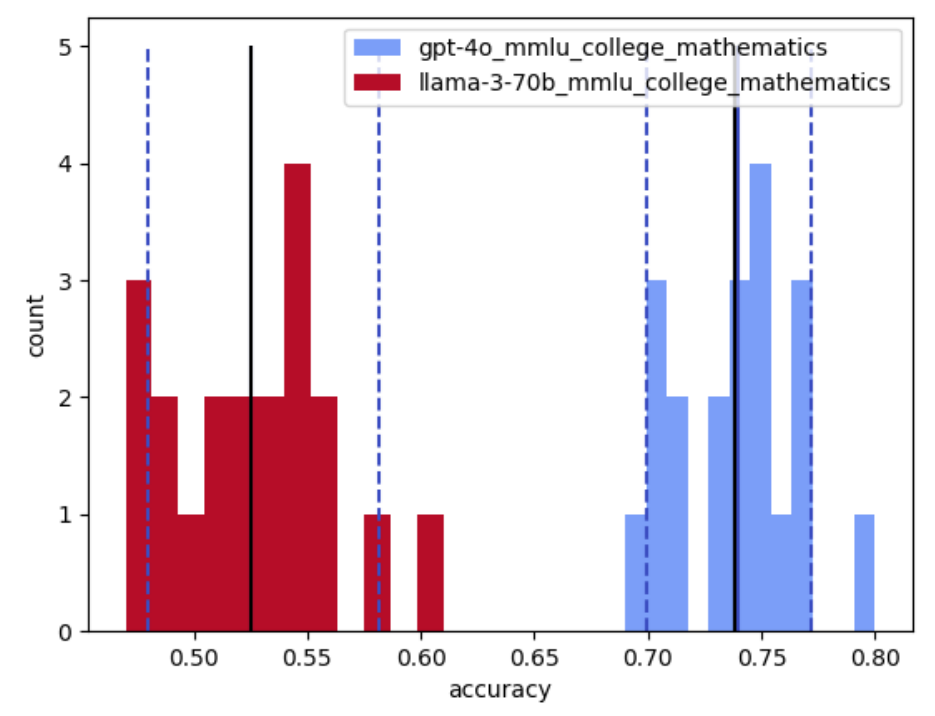
\includegraphics[width=0.7\linewidth]{figures/nondeterminism_accuracy.png}
\caption{Accuracy over 20 identical inference runs on the college mathematics task at $T=0$ \cite{nondeterminism_llm_settings}.}
\label{fig:nondeterminism_accuracy-original}
\end{figure}

These findings demonstrate that deterministic decoding alone is insufficient to guarantee stable or reliable outputs, motivating the need for external validation and control mechanisms.

\subsection{Explainable Artificial Intelligence (XAI) und Trustworthiness.}
Ali et al.\ untersuchen XAI als zentrale Voraussetzung für vertrauenswürdige KI und betonen, dass die Black-Box-Natur vieler moderner Modelle (insbesondere DNNs) die Nachvollziehbarkeit von Entscheidungen und damit das Vertrauen in kritischen Anwendungen erschwert \cite{ali2023xai_trustworthy}.

\begin{figure}[t]
  \centering
  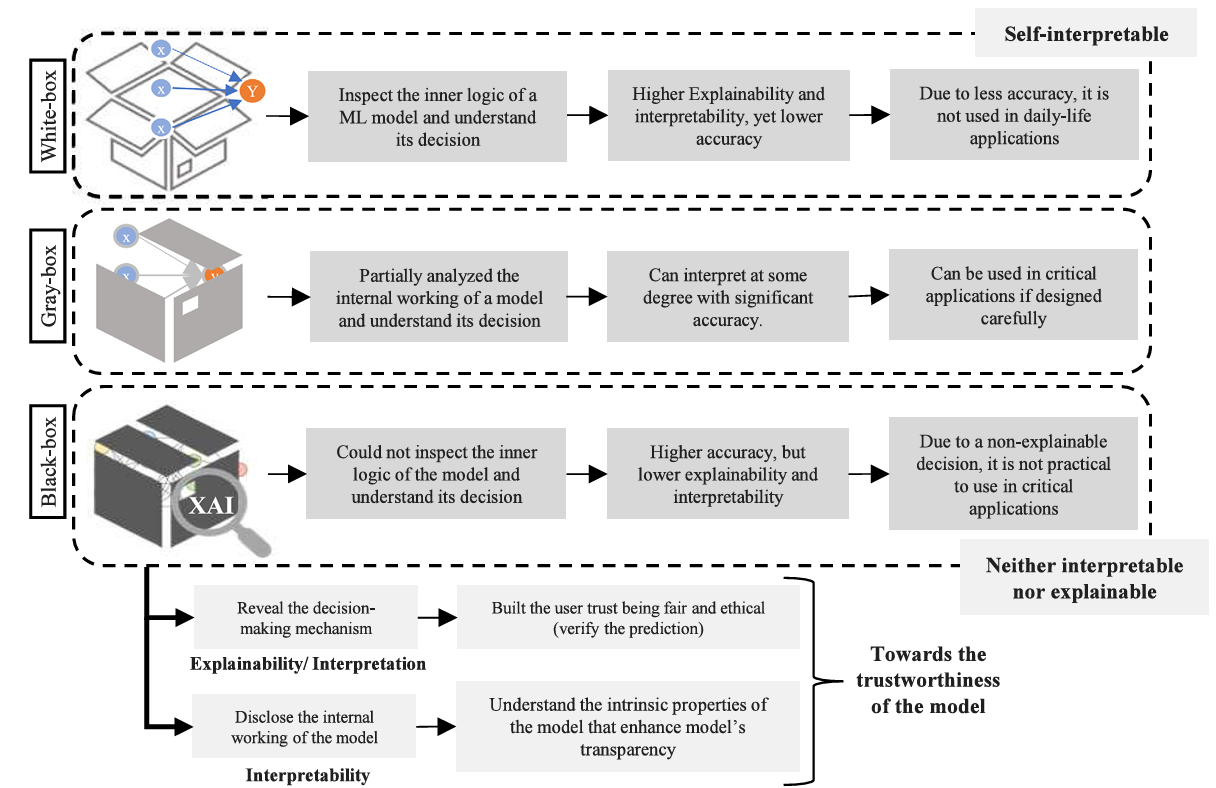
\includegraphics[width=\linewidth]{figures/xai_white_gray_black.png}
  \caption{Vergleich von White-box-, Gray-box- und Black-box-Modellen entlang Interpretierbarkeit/Erklärbarkeit und Genauigkeit. White-box-Modelle sind per Design interpretierbar (höhere Transparenz, typischerweise geringere Genauigkeit), Gray-box-Modelle bieten einen praktikablen Trade-off, während Black-box-Modelle meist hohe Genauigkeit bei geringer Interpretierbarkeit aufweisen und daher zusätzliche XAI-Methoden benötigen, um Vertrauen in kritischen Anwendungen zu unterstützen. (nach Ali et al.)}
  \label{fig:xai_white_gray_black}
\end{figure}

Im Zentrum der Argumentation steht Abb.~\ref{fig:xai_white_gray_black}, die drei Modellklassen entlang eines Interpretierbarkeits--Genauigkeits-Trade-offs gegenüberstellt: \emph{White-box}-Modelle sind per Design interpretierbar und erlauben Einsicht in die interne Entscheidungslogik, werden jedoch als weniger genau charakterisiert und daher selten in alltäglichen Anwendungen eingesetzt. \emph{Gray-box}-Modelle bieten eine Zwischenposition, in der Teile der internen Funktionsweise analysierbar sind und so ein praktikabler Kompromiss zwischen Erklärbarkeit/Interpretierbarkeit und Genauigkeit entsteht, wodurch sie bei sorgfältigem Design auch für kritische Anwendungen in Frage kommen. \emph{Black-box}-Modelle erreichen typischerweise die höchste Genauigkeit, entziehen sich jedoch weitgehend der inneren Inspektion; folglich sind zusätzliche (post-hoc) XAI-Methoden notwendig, um Interpretationen/Erklärungen zu erzeugen und die Nutzung in risikoreichen Szenarien abzusichern. 
Auf Basis dieser Perspektive strukturieren die Autor*innen den XAI-Forschungsraum entlang vier Achsen einer typischen KI-Pipeline: (i) \emph{Data Explainability}, (ii) \emph{Model Explainability}, (iii) \emph{Post-hoc Explainability} und (iv) \emph{Assessment of Explanations}. Diese Einordnung verknüpft methodische XAI-Ansätze mit Evaluationsmetriken, Open-Source-Tooling und offenen Forschungsfragen (z.\,B.\ Systemdesign, Generalisierung, User-Interaktion und Ground-Truth-Evaluation), und rahmt XAI explizit als Mittel, um von reiner Performance-Optimierung hin zu robuster, überprüfbarer Vertrauenswürdigkeit zu gelangen \cite{ali2023xai_trustworthy}.

\subsection{Let´s verify step by step}
\label{subsec:process-supervision-original}

While non-determinism affects output stability, reasoning reliability constitutes a second major challenge.
The study \cite{lets_verify_step_by_step} distinguishes between outcome supervision and process supervision for training reward models.
Outcome-supervised reward models (ORMs) are trained solely on final answers, whereas process-supervised reward models (PRMs) receive feedback at each intermediate reasoning step.

Prior work has shown that outcome-supervised models may reach correct answers through incorrect reasoning paths \cite{lets_verify_step_by_step}.
Process supervision mitigates this misalignment by explicitly penalizing faulty intermediate steps.
The interface used to collect step-level feedback is illustrated in Figure~\ref{fig:process_supervision_interface-original}.

\begin{figure}[h]
\centering
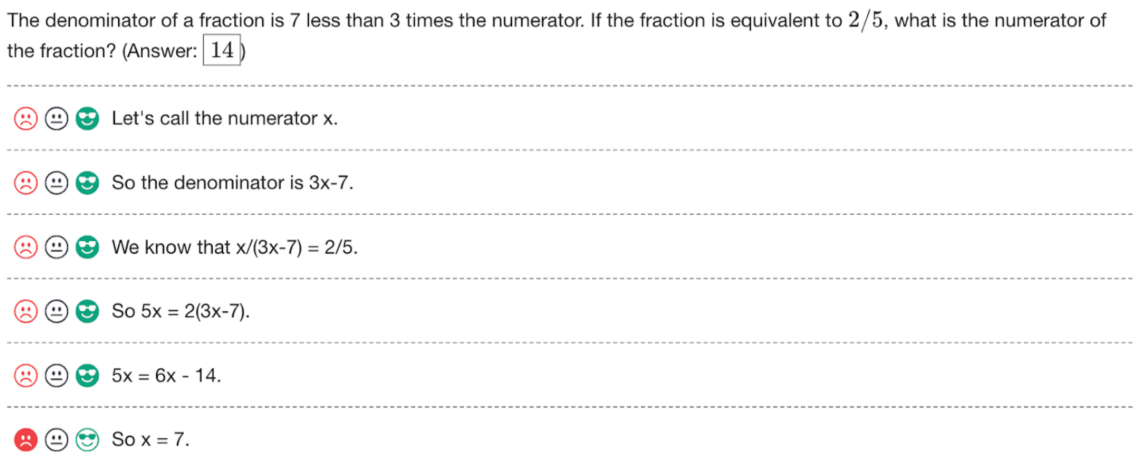
\includegraphics[width=0.7\linewidth]{figures/process_supervision_interface.png}
\caption{Interface for collecting step-level feedback in process supervision \cite{lets_verify_step_by_step}.}
\label{fig:process_supervision_interface-original}
\end{figure}

Empirically, \cite{lets_verify_step_by_step} shows that PRMs substantially outperform ORMs when searching over multiple candidate solutions.
Figure~\ref{fig:prm_vs_orm-original} compares outcome-supervised and process-supervised reward models under varying computational budgets.
Across settings, PRMs consistently solve a higher percentage of problems.

\begin{figure}[h]
\centering
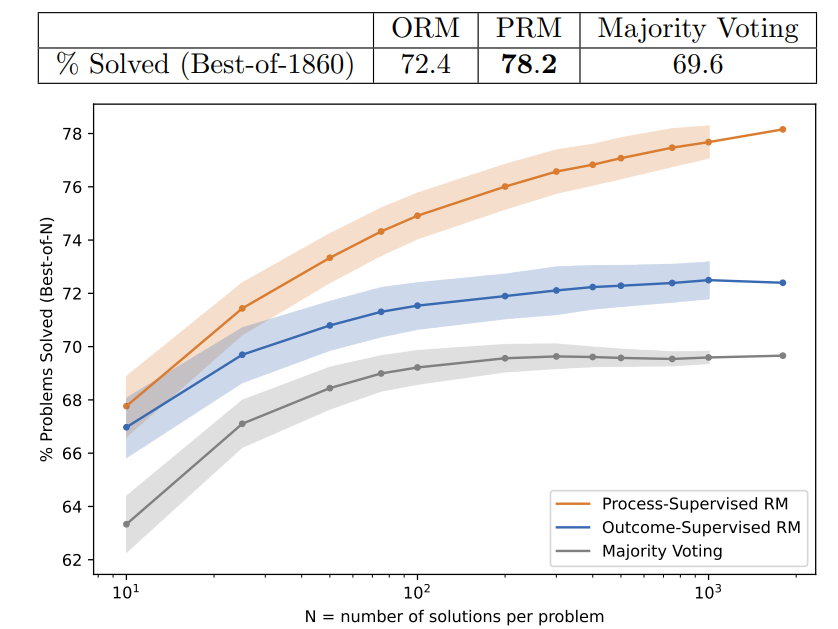
\includegraphics[width=0.7\linewidth]{figures/prm_vs_orm.png}
\caption{Comparison of outcome-supervised and process-supervised reward models \cite{lets_verify_step_by_step}.}
\label{fig:prm_vs_orm-original}
\end{figure}

Using a representative subset of the MATH benchmark, the authors report that their process-supervised model solves 78.2\% of problems.
Additional experiments demonstrate that large reward models can approximate human supervision and that active learning improves data efficiency by a factor of 2.6.
The PRM800K dataset is released to support further research.

Despite these advances, process supervision remains probabilistic and training-intensive, and does not provide formal guarantees on individual outputs.

\subsection{Chain-of-Verification for Hallucination Reduction}
\label{subsec:cove-original}

A complementary line of work focuses on hallucination reduction through self-verification.
Hallucinations, defined as plausible but factually incorrect generations \cite{chain_of_verification}, become more prevalent in long-form generation due to exposure bias.
Chain-of-Verification (CoVe) addresses this issue by decomposing verification into multiple explicit steps.

As illustrated in Figure~\ref{fig:cove_overview-original}, CoVe operates by first generating a baseline response, then planning verification questions, answering these questions independently, and finally producing a revised response that incorporates verification results.

\begin{figure}[h]
\centering
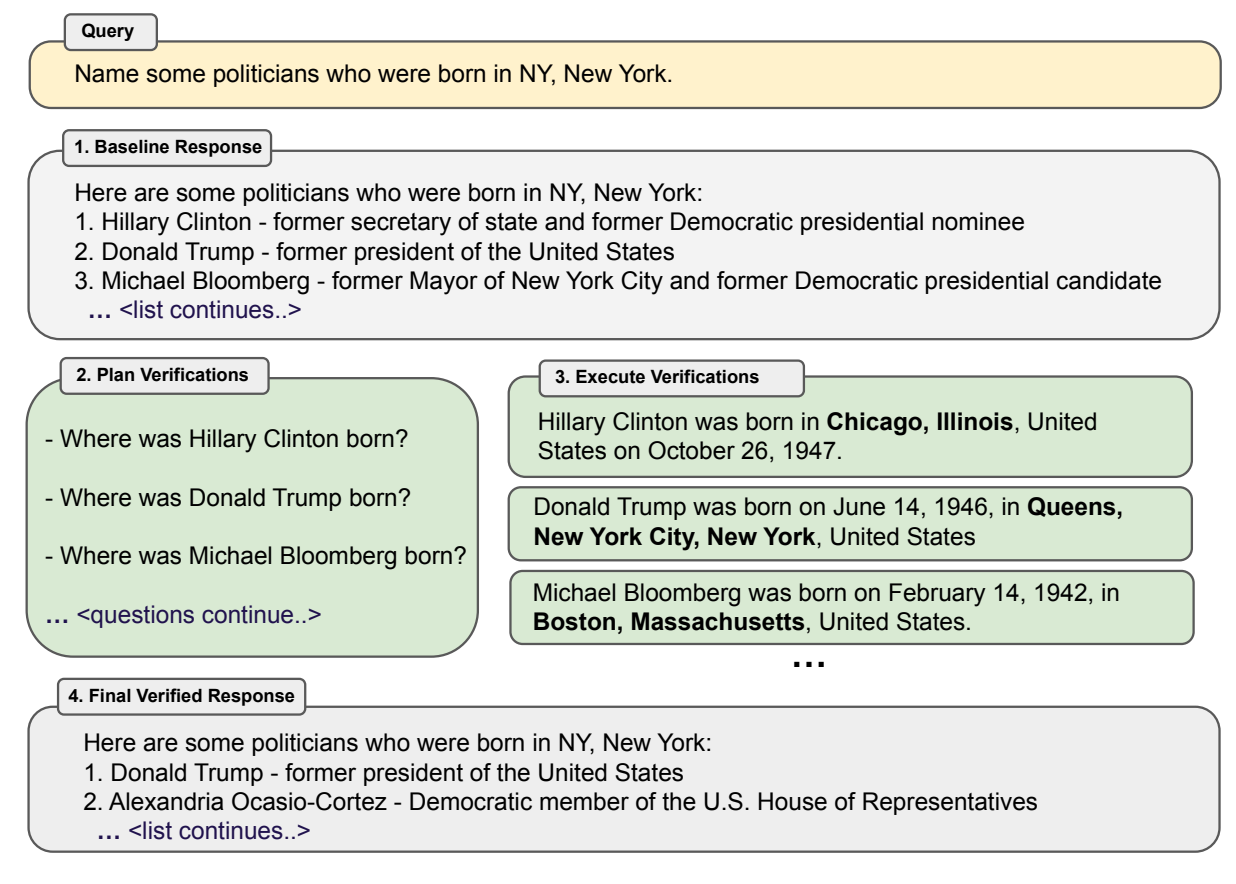
\includegraphics[width=0.8\linewidth]{figures/cove_overview.png}
\caption{Overview of the Chain-of-Verification (CoVe) method \cite{chain_of_verification}.}
\label{fig:cove_overview-original}
\end{figure}

Experiments across multiple benchmarks demonstrate that CoVe reduces hallucination rates without significantly decreasing correct content.
Table~\ref{tab:cove_wikidata} reports precision improvements on list-based Wikidata and Wiki-Category tasks, while Table~\ref{tab:cove_multispanqa} shows improved F1 scores on closed-book MultiSpanQA.
Long-form biography generation results, summarized in Table~\ref{tab:cove_longform}, further confirm substantial gains in factual accuracy.

While CoVe significantly improves generation quality, the authors explicitly note that hallucinations are not fully eliminated.
Thus, CoVe should be understood as a probabilistic mitigation strategy rather than a guarantee mechanism.
